\chapter{Ανάπτυξη Διαδικτυακής Εφαρμογής iBoot}
Σε αυτό το κεφάλαιο, αναλύονται οι λειτουργίες που παρέχει η διαδικτυακή εφαρμογή στους χρήστες της μέσω Διεπαφής Χρήστη (User Interface) και παρέχεται επεξήγηση των αρχείων κώδικα, ο οποίος συντέλεσε στη δημιουργία του πληροφοριακού συστήματος. Ανάλογα με τον ρόλο του χρήστη που συνδέεται στην εφαρμογή, παρέχονται και οι αντίστοιχες λειτουργίες. Η εμφάνιση της εφαρμογής έχει ίδια αισθητικά χαρακτηριστικά για κάθε είδος χρήστη. Το User Interface θεωρείται από τα πιο σημαντικά μέρη μιας διαδικτυακής εφαρμογής καθώς, αν είναι σχεδιασμένο σωστά, ώστε να είναι εύχρηστο και διαισθητικό, κάνει εύκολη τη χρήση των λειτουργιών του συστήματος, ακόμη και σε χρήστες που πιθανώς δεν είναι εξειδικευμένοι στον τομέα της πληροφορικής.

Για την κατασκευή του User Interface, χρησιμοποιήθηκε η αρχή του Reactive Programming, δηλαδή της μεθόδου προγραμματισμού ιστού ώστε το περιεχόμενο της εφαρμογής να ανανεώνεται δυναμικά και ασύγχρονα με τις ενέργειες του χρήστη, σε ένα εν γένει στατικό περιβάλλον. Όσον αφορά το σχεδιασμό του γραφικού περιβάλλοντος, χρησιμοποιήθηκε Responsive Design, ώστε η εφαρμογή να έχει ομοιόμορφη, καλαίσθητη και λειτουργική εμφάνιση, τόσο σε συσκευές με μεγάλη διάμετρο οθόνης, όπως ηλεκτρονικούς υπολογιστές, όσο και σε συσκευές με μικρότερη διάμετρο οθόνης, όπως κινητά τηλέφωνα. Ο συνδυασμός των παραπάνω μεθόδων προγραμματισμού ιστού, προσφέρει ευχάριστη εμπειρία χρήσης της εφαρμογής, σε όλους τους χρήστες, ανεξάρτητα από τον τύπο συσκευής που χρησιμοποιούν.

Η διαδικτυακή εφαρμογή έχει υλοποιηθεί ως ένα γραφικό περιβάλλον ιστού που επικοινωνεί με τη βάση δεδομένων του μέσω ενός Restful API. Για την ανάπτυξη της εφαρμογής έγινε χρήση του CodeIgniter PHP Framework. Η αναλυτική προδιαγραφή του API που παρέχει η πλατφόρμα, μετά την εγκατάσταση της, δημιουργήθηκε με χρήση του Swagger UI και βρίσκεται στην τοποθεσία \texttt{/api} και περιγράφει όλες τις λειτουργίες που είναι δυνατό να πραγματοποιηθούν με τη χρήση του.

\section{Διεπαφή Χρήστη}

\subsection{Εγγραφή \& Σύνδεση στο Σύστημα}

\FloatBarrier

\begin{figure}[ht]
	\centering
	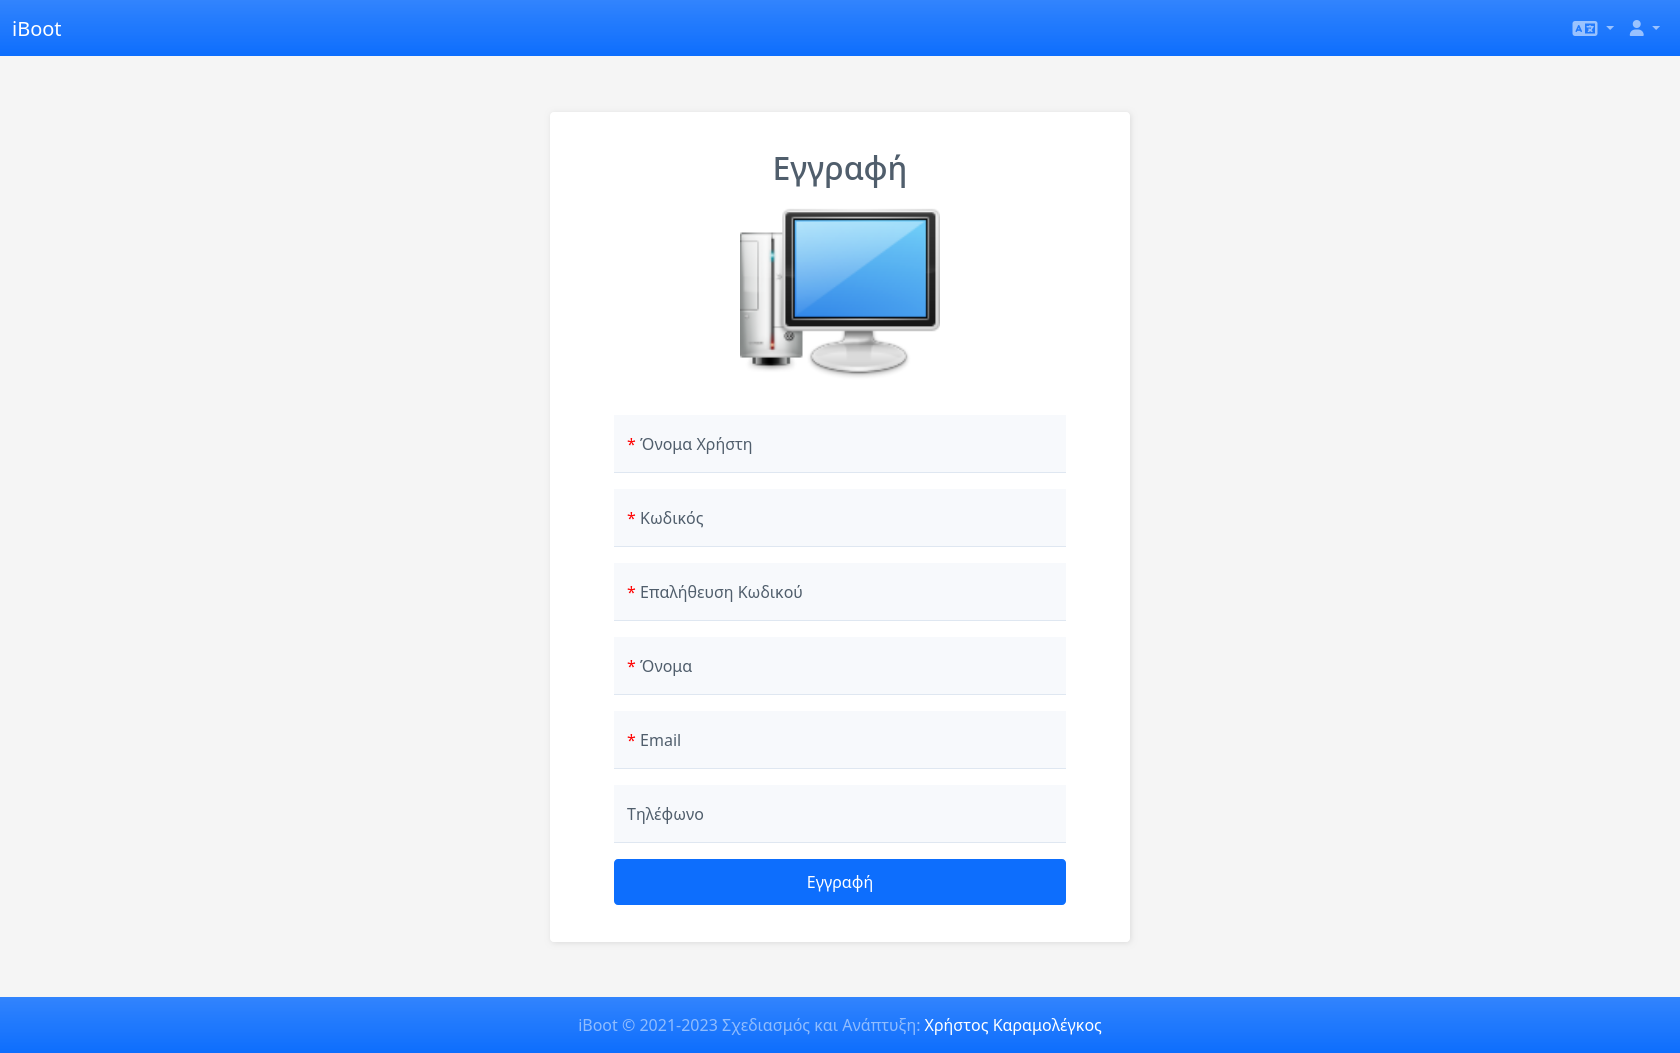
\includegraphics[scale=0.25]{iBoot-register.png}
	\caption{iBoot - Εγγραφή}
	\label{fig:iBoot_register}
\end{figure}

\begin{figure}[ht]
	\centering
	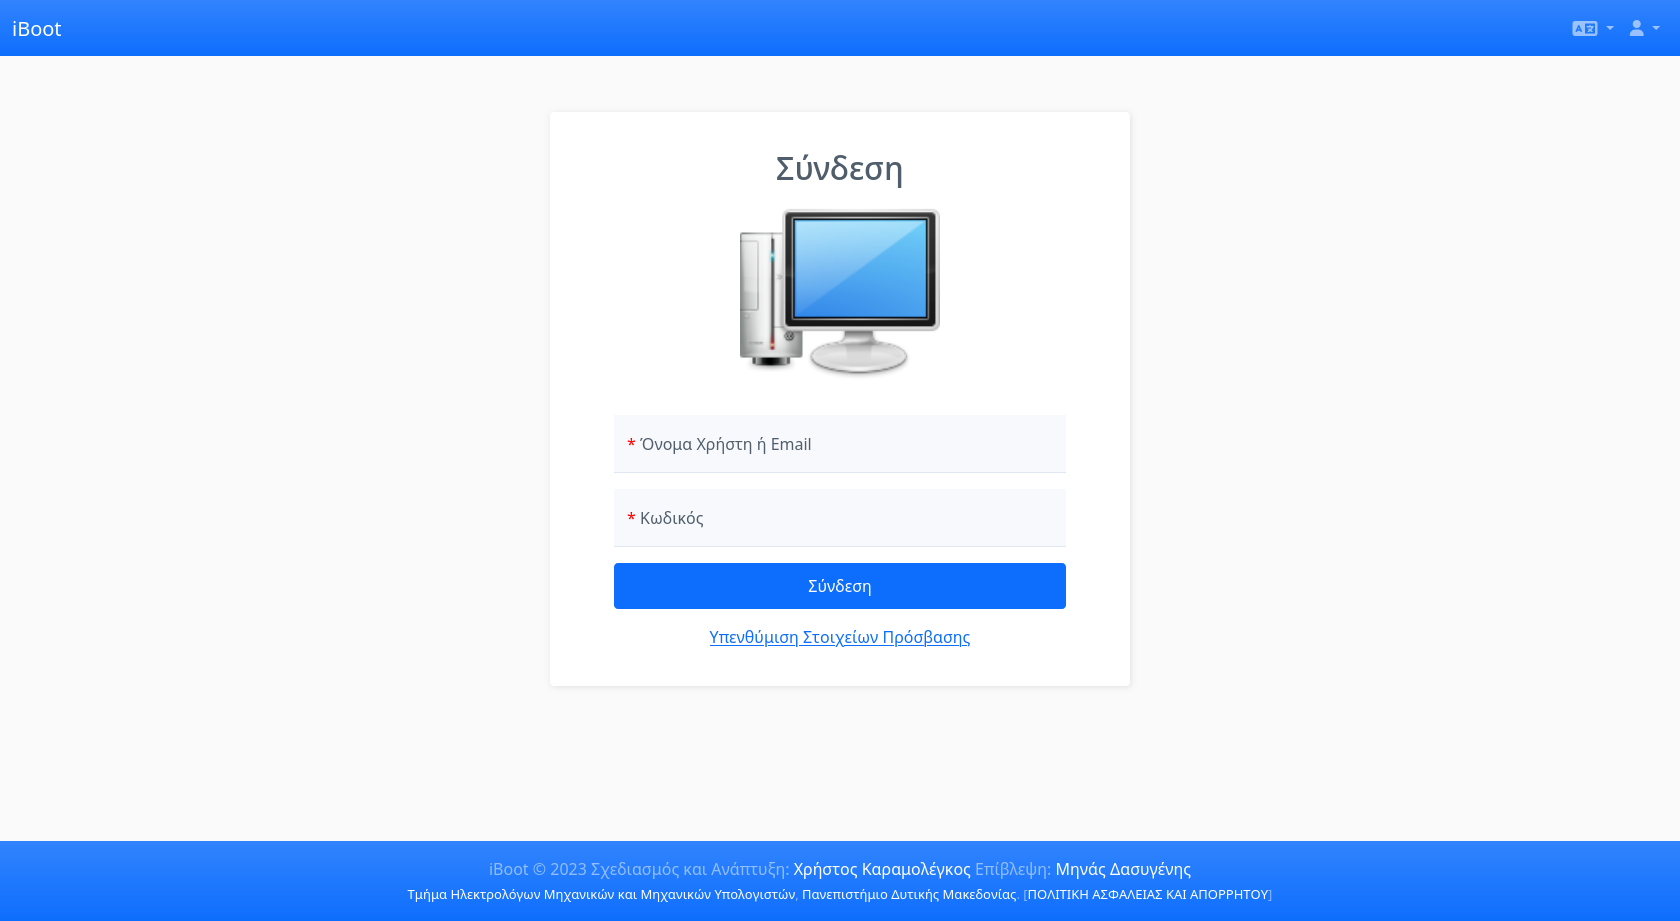
\includegraphics[scale=0.25]{iBoot-login.png}
	\caption{iBoot - Σύνδεση}
	\label{fig:iBoot_login}
\end{figure}

\begin{figure}[ht]
	\centering
	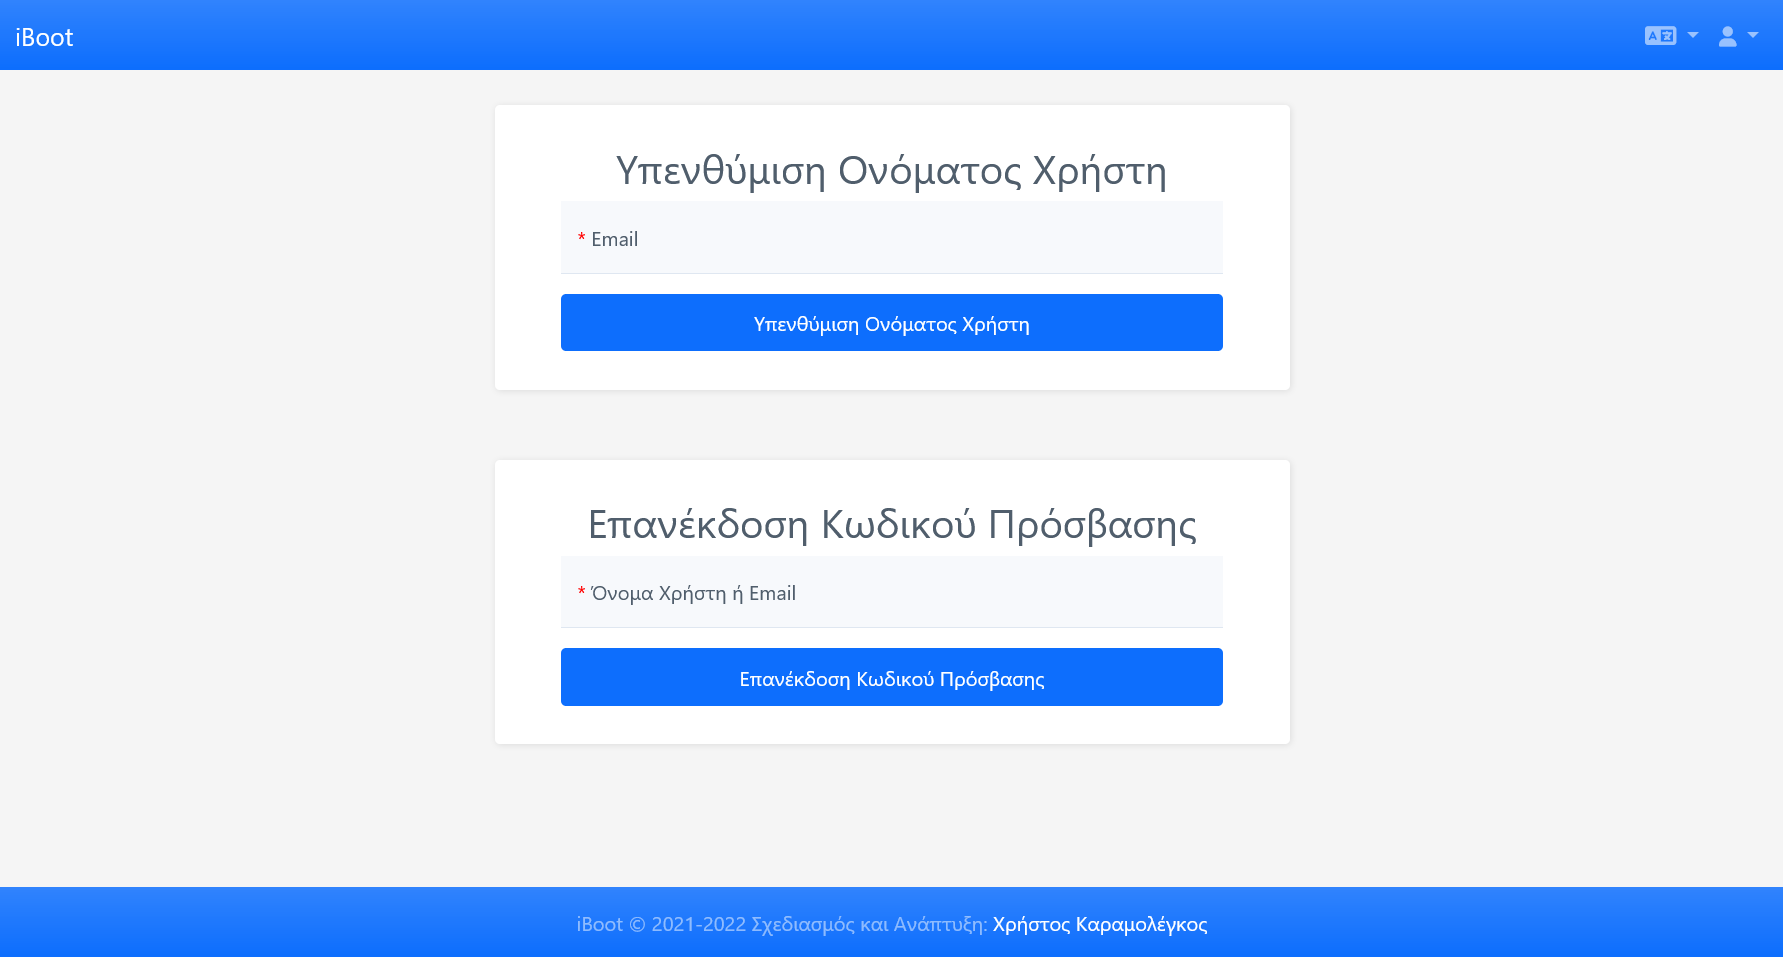
\includegraphics[scale=0.25]{iBoot-forgot-credentials.png}
	\caption{iBoot - Υπενθύμιση Στοιχείων Πρόσβασης}
	\label{fig:iBoot_forgot_credentials}
\end{figure}

\FloatBarrier

\subsection{Μενού Πλοήγησης}

\subsection{Υπολογιστές}

\subsection{Ομάδες Υπολογιστών}

\subsection{Εργαστήρια}

\subsection{Block εντολών τύπου ipxe}

\subsection{Μενού Εκκίνησης}

\subsection{Χρονοδιαγράμματα}

\subsection{Προδιαγραφή API}

\section{Επεξήγηση Αρχείων}
Καθώς η διαδικτυακή εφαρμογή αναπτύχθηκε με χρήση του CodeIgniter 4 Framework, χρησιμοποιεί και τη δομή αρχείων του\cite{CodeIgniter_structure}.

\subsection{Βασική Δομή}
Η βασική δομή της εφαρμογής αποτελείται από πέντε καταλόγους: \hyperref[ui:app]{app/}, \hyperref[ui:public]{public/}, \hyperref[ui:writable]{writable/}, \hyperref[ui:tests]{tests/} και \hyperref[ui:system]{vendor/ ή system/}.

\subsubsection{app} \label{ui:app}
Στον κατάλογο app βρίσκεται όλος ο κώδικας της εφαρμογής. Οι ακόλουθοι φάκελοι αποτελούν τα βασικά περιεχόμενα:\\

{\footnotesize
\begin{forest}
	for tree={
		font=\ttfamily,
		grow'=0,
		child anchor=west,
		parent anchor=south,
		anchor=west,
		calign=first,
		inner xsep=7pt,
		edge path={
			\noexpand\path [draw, \forestoption{edge}]
			(!u.south west) +(7.5pt,0) |- (.child anchor) pic {folder} \forestoption{edge label};
		},
		before typesetting nodes={
			if n=1
			{insert before={[,phantom]}}
			{}
		},
		fit=band,
		before computing xy={l=15pt},
	}  
	[app/
		[Config/ \ \ \ \ \ \ Αρχεία ρύθμισης παραμέτρων της εφαρμογής]
		[Controllers/ \ Οι Controllers που καθορίζουν τη ροή του προγράμματος]
		[Database/ \ \ \ \ Κλάσεις για την ενημέρωση του σχήματος και την αρχικοποίηση βάσεων δεδομένων]
		[Filters/ \ \ \ \ \ Κλάσεις φίλτρων που μπορούν να εκτελούνται πριν και μετά τους controllers]
		[Helpers/ \ \ \ \ \ Συλλογές αυτόνομων βοηθητικών συναρτήσεων]
		[Language/ \ \ \ \ Συμβολοσειρές γλώσσας για την υποστήριξη πολλαπλών γλωσσών]
		[Libraries/ \ \ \ Χρήσιμες κλάσεις που δεν ταιριάζουν σε άλλη κατηγορία]
		[Models/ \ \ \ \ \ \ Τα Models που διασυνδέουν την εφαρμογή με τη βάση δεδομένων]
		[ThirdParty/ \ \ Βιβλιοθήκες τρίτων που μπορούν να χρησιμοποιηθούν στην εφαρμογή]
		[Views/ \ \ \ \ \ \ \ Τα Views που συνθέτουν την HTML που εμφανίζεται στον πελάτη]
	]
\end{forest}
}

Στον κατάλογο app έχει δοθεί το php namespace 'iBoot', έτσι ώστε τα ονόματα των αρχείων που βρίσκονται στους υποκαταλόγους του να μην συγκρούονται με ομοίως ονομαζόμενα αρχεία του Framework ή άλλων χρησιμοποιούμενων βιβλιοθηκών.

\subsubsection{public} \label{ui:public}
Ο κατάλογος public περιέχει το προσβάσιμο από το πρόγραμμα περιήγησης τμήμα της διαδικτυακής εφαρμογής, αποτρέποντας την άμεση πρόσβαση στον πηγαίο κώδικα. Περιέχει το κύριο αρχείο .htaccess, το index.php και όλα τα επιπρόσθετα στοιχεία της εφαρμογής, όπως CSS, javascript και εικόνες.

Αυτός ο φάκελος προορίζεται να είναι η "διαδικτυακή ρίζα" της εφαρμογής και ο διακομιστής ιστού θα πρέπει να ρυθμιστεί ώστε να δείχνει σε αυτόν.

\subsubsection{writable} \label{ui:writable}
Αυτός ο κατάλογος περιέχει όλους τους καταλόγους στους οποίους μπορεί να χρειαστεί να γίνει εγγραφή αρχείων κατά τη διάρκεια της ζωής της εφαρμογής. Αυτό περιλαμβάνει καταλόγους για την αποθήκευση προσωρινών αρχείων cache, αρχείων καταγραφής συμβάντων και τυχόν μεταφορτώσεις που μπορεί να στείλει ένας χρήστης. Θα πρέπει να προστεθούν εκεί όλοι οι κατάλογοι στους οποίους θα χρειαστεί να γράψει η εφαρμογή. Αυτό επιτρέπει τον ορισμό των υπόλοιπων κύριων καταλόγων ως μη εγγράψιμους, ως πρόσθετο μέτρο ασφαλείας κατά της ανεπιθύμητης τροποποίησης του κώδικα της εφαρμογής.

\subsubsection{tests} \label{ui:tests}
Αυτός ο κατάλογος έχει οριστεί για να περιέχει τα αρχεία δοκιμών. Ο κατάλογος \_support περιέχει διάφορες κλάσεις προσομοίωσης και άλλα βοηθητικά προγράμματα που μπορούν να χρησιμοποιηθούν για τη συγγραφή και εκτέλεση δοκιμών. Αυτός ο κατάλογος δεν χρειάζεται να υπάρχει στην παραγωγική εγκατάσταση της εφαρμογής.

\subsubsection{system} \label{ui:system}
Αυτός ο κατάλογος περιέχει τα αρχεία που συνθέτουν το ίδιο το CodeIgniter 4 Framework. Tα αρχεία στον κατάλογο συστήματος δεν πρέπει ποτέ να τροποποιούνται. Αντ' αυτού, μπορούν να επεκταθούν οι υπάρχουσες κλάσεις ή να δημιουργήθούν νέες, ώστε να παρέχουν την επιθυμητή λειτουργικότητα.

Όλα τα αρχεία σε αυτόν τον κατάλογο βρίσκονται κάτω από το php namespace `CodeIgniter'.

Η εγκατάσταση του framework έχει γίνει με τη βοήθεια του Composer, οπότε στην περίπτωσή μας, ο κατάλογος συστήματος βρίσκεται στη διαδρομή `vendor/codeigniter4/framework/system'.

\section{Ασφάλεια Συστήματος}

\section{Σύνοψη Κεφαλαίου 4}
Στο κεφάλαιο 4, εξετάστηκαν όλες οι δυνατότητες της διαδικτυακής εφαρμογής και τα βήματα που πρέπει να ακολουθήσει ένας νέος χρήστης για να τις χρησιμοποιήσει. Επιπλέον, παρασχέθηκε οπτικό υλικό για κάθε λειτουργία στην οποία εμφανιζόταν στον χρήστη η διεπαφή χρήστη της διαδικτυακής εφαρμογής κατά την πλοήγησή του. Στη συνέχεια, εξηγήθηκαν διεξοδικά τόσο το front-end όσο και το back-end της δομής του πληροφοριακού συστήματος. Προκειμένου να διασφαλιστεί η ασφάλεια κατά τη χρήση της διαδικτυακής εφαρμογής, παρέχεται επεξήγηση των πρωτοκόλλων και των προσεγγίσεων ασφαλείας.

Στο επόμενο κεφάλαιο θα γίνει αξιολόγηση του συστήματος, ως προς την ορθή λειτουργία του και τις δυνατότητες κλιμάκωσής του.
